\chapter{面向国产异构处理器的移植工作}
\label{面向国产异构处理器的移植工作}

\section{华为昇腾910硬件架构}
\label{华为昇腾910硬件架构}

华为昇腾910加速卡包含34个基于``达芬奇''架构的AI Core,负责执行向量和张量相关的计算密集型算子。\footnote{\url{https://support.huawei.com/enterprise/zh/doc/EDOC1100164829/f96da97d}}不同于传统的支持通用计算的CPU 和GPU,也不同于专用于某种特定算法的专用芯片ASIC,达芬奇架构本质上是为了适应某个特定领域中的常见应用和算法,通常称为DSA(Domain Specific Architecture,特定域架构)芯片。

\begin{figure}[h]
    \centering
    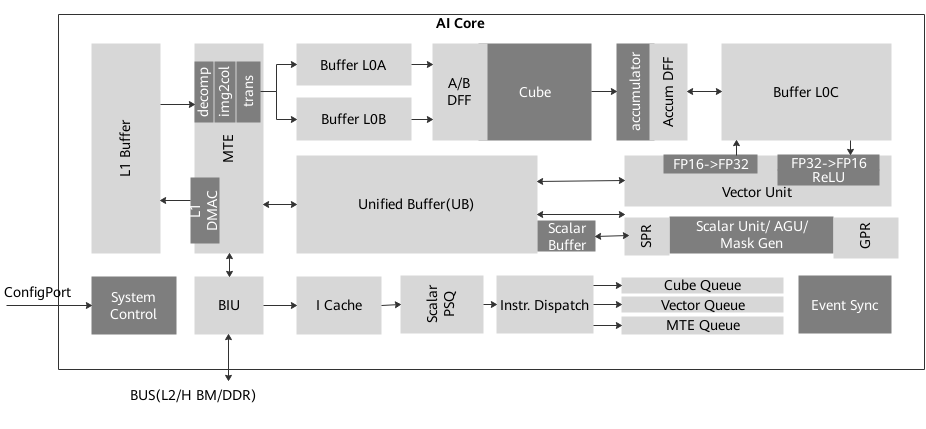
\includegraphics[width=1\textwidth]{image/chap03/davinci.png}
    \caption{达芬奇架构图}
    \label{达芬奇架构图}
\end{figure}

达芬奇架构如\autoref{达芬奇架构图}所示,从控制上可以看成是一个相对简化的现代微处理器的基本架构。它包括了三种基础计算资源: 矩阵计算单元(Cube Unit)、向量计算单元(Vector Unit)和标量计算单元(Scalar Unit)。这三种计算单元分别对应了张量、向量和标量三种常见的计算模式,在实际的计算过程中各司其职,形成了三条独立的执行流水线,在系统软件的统一调度下互相配合达到优化的计算效率。此外在矩阵计算单元和向量计算单元内部还提供了不同精度、不同类型的计算模式。

\subsection{计算单元}

AI Core中的执行单元主要包括:Cube,Vector和Scalar,完成AI Core中不同类型的数据计算。

当前,华为并没有对外开放Cube单元的自定义算子开发方式。因此,要发挥Cube算子的半精度算力,只能调用CANN软件包内置的 \lstinline{MatMul}、\lstinline{MatMulV2} 或 \lstinline{GEMM} 等算子。

\subsection{存储单元}

AI Core中存在内部存储,AI Core需要把外部存储中的数据加载到内部存储中,才能完成相应的计算。AI Core的内部存储包括:L1 Buffer、L0 Buffer、Unified Buffer、GPR(General-Purpose Register,通用寄存器),SPR(Special-Purpose Register,专用寄存器)和Scalar Buffer。

为了配合AI Core中的数据传输和搬运,AI Core中还包含BIU(Bus Interface Unit),MTE1(Memory Transfer Engine,内存传输引擎),MTE2,MTE3。其中BIU为AI Core与总线交互的接口;MTE为数据搬运单元,完成不同Buffer之间的数据搬运。

\subsection{控制单元}

AI Core中的控制单元主要包括:系统控制模块(System Control),标量指令处理队列(Scalar PSQ),指令发射模块(Instr. Dispatch),矩阵运算队列(Cube Queue),向量运算队列(Vector Queue),存储转换队列(MTE Queue)和事件同步模块(Event Sync)。

系统控制模块负责指挥和协调AI Core的整体运行模式,配置参数和实现功耗控制等。

标量指令处理队列主要实现控制指令的译码,如果指令是标量指令,指令会被直接执行;否则根据指令的不同类型,将会分别被指令发射模块顺次发射到矩阵运算队列、向量运算队列和存储转换队列,然后再分配到某个空间的执行部件进行执行。

除标量队列之外,分属于不同队列的指令能够乱序执行,但是队列内部指令为顺序执行,即在满足数据依赖的前提下,指令的物理执行顺序不一定与代码的书写顺序一致。

\section{AscendCL编程模型}

\begin{wrapfigure}{r}{0.5\linewidth}
    \centering
    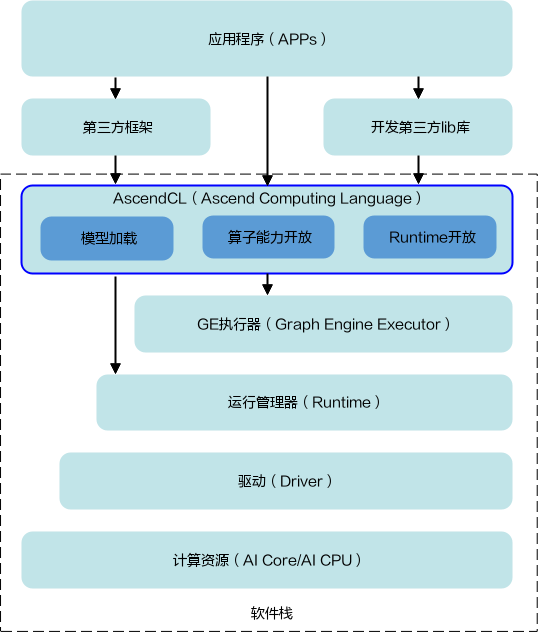
\includegraphics[width=0.5\textwidth]{image/chap03/AscendCL}
    \caption{AscendCL逻辑架构图}
    \label{AscendCL逻辑架构图}
\end{wrapfigure}

\footnote{\url{https://support.huawei.com/enterprise/zh/doc/EDOC1100164875/b6db6b40}}AscendCL(Ascend Computing Language)提供Device管理、Context管理、Stream管理、内存管理、模型加载与执行、算子加载与执行、媒体数据处理等C语言API库供用户开发深度神经网络应用,用于实现目标识别、图像分类等功能。用户可以通过第三方框架调用AscendCL接口,以便使用昇腾AI处理器的计算能力;用户还可以使用AscendCL封装实现第三方lib库,以便提供昇腾AI处理器的运行管理、资源管理能力。

在运行应用时,AscendCL调用GE执行器提供的接口实现模型和算子的加载与执行、调用运行管理器的接口实现Device管理/Context管理/Stream管理/内存管理等。

计算资源层是昇腾AI处理器的硬件算力基础,主要完成神经网络的矩阵相关计算、完成控制算子/标量/向量等通用计算和执行控制功能、完成图像和视频数据的预处理,为深度神经网络计算提供了执行上的保障。

\autoref{AscendCL逻辑架构图}给出了AscendCL逻辑架构图。

\section{移植方案}

\subsection{将GEMM拆分为更细粒度的MatMul}

由\autoref{AscendCL接口与算子调用实验}的Profile实验可知,在昇腾910上GEMM算子性能远低于MatMulV2。这使得我们有必要拆解HPL-AI中的GEMM过程:$C\leftarrow\alpha AB+\beta C$,将其中$\alpha$、$\beta$的系数乘法和矩阵加法过程移动到CPU上完成。由于这两个过程都是$O(n^2)$的时间复杂度,因此不会带来过大的额外开销。

此外在我们实现的HPL-AI(及HPL标准实现)中,对gemm的调用都有$\alpha=-1,\beta=1$,因此对于$\beta$的系数乘法过程可以省略,这样运行时的开销再次减少了。

\subsection{基于矩阵分块的负载均衡算法}
\label{基于矩阵分块的负载均衡算法}

我们使用了基于\autoref{分块矩阵乘法公式}的矩阵分块方法,将计算量均匀负载到CPU和异构处理器上。

\begin{equation}
    \begin{split}
        \label{分块矩阵乘法公式}
        \begin{bmatrix}
            A_{1,1} & A_{1,2} \\
            A_{2,1} & A_{2,2}
        \end{bmatrix}
        \begin{bmatrix}
            B_{1,1} & B_{1,2} \\
            B_{2,1} & B_{2,2}
        \end{bmatrix}
        &=\begin{bmatrix}
            A_{1,1}B_{1,1}+A_{1,2}B_{2,1} & A_{1,1}B_{1,2}+A_{1,2}B_{2,2} \\
            A_{2,1}B_{1,1}+A_{2,2}B_{2,1} & A_{2,1}B_{1,2}+A_{2,2}B_{2,2}
        \end{bmatrix} \\
        &= \begin{bmatrix}
            C_{1,1} & C_{1,2} \\
            C_{2,1} & C_{2,2}
        \end{bmatrix}
    \end{split}
\end{equation}

我们设定了一个参数$P=2048$,用于控制CPU在矩阵乘法中的负载。对于输入为$\left(M,N,K\right)$的矩阵乘法,取$\left(M_2,N_2,K_2\right)=\left(M \mod P,N\mod P,K\mod P\right)$,$\left(M_1,N_1,K_1\right)=\left(M-M_2,N-N_2,K-K_2\right)$,我们将规模为$\left(M_1,N_1,K_1\right)$的子矩阵乘法$A_{1,1}B_{1,1}$放在异构处理器上,其余运算放在CPU上。容易发现,除了一个规模非常小的矩阵乘法$A_{1,2}B_{2,1}$过程外,其余3个子矩阵乘法$C_{1,2},C_{2,1},C_{2,2}$求解都是可以和异构处理器上的乘法过程同步执行的,这样就实现了CPU和异构处理器的负载均衡。

这种负载分配还带来了另外一个好处:在异构处理器上的问题规模总是$P$的整数倍,可以使内存对齐以充分利用异构处理器的高算力,同时也将需要编译的算子至多减少$P\times P$倍。

\subsection{数据打包与转置}
\label{数据打包与转置}

在BLAS提供的接口中,一个矩阵$A$通常由$M,N,\mathit{LDA}$三个参数确定其在内存中的分布,分别表示矩阵的行、列,及相邻两行同列元素的跨度(假设矩阵表示为row-major)。这样设计可以方便提取子矩阵,同时也更容易利用内存对齐优化运行时开销。

然而,昇腾910是专门为AI场景设计的加速卡,其输入格式只支持张量(Tensor)格式,或是其他非通用矩阵格式\footnote{尤为尴尬的是,AscendCL中提供的GEMM封装,不但性能远低于手动调用MatMulV2,同时只支持$LDA=-1$的输入,即二维张量,可理解为row-major形式下$\mathit{LDA}=N$的矩阵}。不考虑这种设计的好坏,如果要将CPU上的通用矩阵移动到NPU上并进行计算,只有如下两种选择:

\begin{itemize}
    \item 因为当前AscendCL中并没有像CUDA一样提供二维拷贝的接口,我们需要(不妨假设为row-major的表示方式)向设备逐行 \lstinline{aclrtMemcpyAsync},在矩阵行数较多时会有很多调用开销。当然这个过程可以使用多流执行,但也会引入额外的抢占开销。
    \item 先在CPU端打包成二维张量格式,然后一次性 \lstinline{aclrtMemcpyAsync}。
\end{itemize}

一开始,我们倾向于使用前一种方案,因为它不需要额外的打包过程。但是,后来我们发现,虽然 \lstinline{MatMul} 和 \lstinline{MatMulV2} 算子提供了编译时可选的属性,标记输入矩阵是否为转置,但设置为转置时编译时就会报错。因此,对于转置的输入,我们只能额外将其重新转置成正常的矩阵。

我们将转置和CPU上的打包合并到一起,如果需要转置则调用\lstinline{latcpy},否则调用\lstinline{lacpy},这两个过程都可以使用多线程的 \lstinline{blas::copy} 加速,从而尽量减少多余的开销。

同理,由于结果矩阵总是非转置的,我们可以一次性将其从设备上拷贝回内存,并多次调用\lstinline{blas::axpy},将其加回原先的矩阵$C$。

\subsection{精度转换}

通过\autoref{数据打包与转置}中的方法,我们将问题转换成对设备上的两个非转置的单精度二维张量做矩阵乘法。因为由\autoref{AscendCL接口与算子调用实验}可知,昇腾910的FP32算力要比FP16低几个数量级,因此我们需要通过 \lstinline{Cast} 算子将其转换成FP16张量格式,并在矩阵乘法结束后重新转回FP32。

\subsection{优化的内存排布}

我们实现了一个优化的内存排布,用于减少设备上的空间占用。\autoref{内存排布图示}给出这种排布的图示。图中hA表示FP16格式的A矩阵,sA表示FP32格式的A矩阵,其他同理。

\begin{figure}[h]
    \centering
    \begin{tabular}{cccccc}
        \cline{1-5}
        \multicolumn{1}{|c|}{}           & \multicolumn{1}{c|}{hB} & \multicolumn{1}{c|}{hA} & \multicolumn{1}{c|}{sA} & \multicolumn{1}{c|}{sB} & Copy+Cast阶段 \\ \cline{1-5}
        \multicolumn{5}{c}{$\downarrow$} &                                                                                                                       \\ \cline{1-5}
        \multicolumn{1}{|c|}{hC}         & \multicolumn{1}{c|}{hB} & \multicolumn{1}{c|}{hA} & \multicolumn{2}{c|}{}   & MatMul阶段                              \\ \cline{1-5}
        \multicolumn{5}{c}{$\downarrow$} &                                                                                                                       \\ \cline{1-5}
        \multicolumn{1}{|c|}{hC}         & \multicolumn{4}{c|}{sC} & Cast+Copy阶段                                                                               \\ \cline{1-5}
    \end{tabular}
    \caption{内存排布图示}
    \label{内存排布图示}
\end{figure}

根据\autoref{LU分解的并行化}的分析,在HPL/HPL-AI中会有很多形如$\left(M,N,K\right),K\ll M,K\ll N$的矩阵乘法调用,我们的排布可以显著减少这种情况下需要的设备内存空间。

\subsection{懒释放}
\label{懒释放}

在异构计算时通常需要在设备上额外分配一块存储空间,并在计算结束时手动将其释放。但是,由\autoref{AscendCL接口与算子调用实验}可知,在NPU上 \lstinline{aclrtMalloc} 和 \lstinline{aclrtFree} 的时间开销都非常大,如果在每次矩阵乘法前后都要分配和释放设备上的空间,将极大影响算法效率。

因此,我们设计了一种被称作``懒释放''(Lazy Free)的策略。在结束一次设备上的计算时,我们并不将这块设备上的空间释放掉,而是记录下本次申请的空间的大小。在下一次启动设备上的计算时,先计算本次计算需要设备空间的大小,如果不超过之前的记录值,则直接使用之前分配的空间;否则释放前一次的空间,并为本次计算重新申请足够的空间。

容易知道,在懒释放策略下,程序申请的空间是单调递增的,并且总是恰好能满足本次计算的需要,只在必须的情况下才会涉及设备空间的释放和重新申请。在程序结束运行时,会统一释放之前申请的空间,且这部分时间无需计入运行结果,这符合HPL-AI基准规则。

当然此策略也可用于CPU上的内存分配过程,但CPU上 \lstinline{malloc} 调用通常比较快,效果并不是那么明显。

\subsection{热身运行}
\label{热身运行}

在单次运行中,\autoref{懒释放}中的策略并不足以完全消除设备空间申请和释放的开销。因此,我们引入热身运行,在运行HPL-AI基准时以完全相同的参数重复运行程序,这样空间申请和释放将只发生在算法的首次运行;对于后续的测试来说,空间申请和释放的开销被完全消除。

这同样符合HPL-AI基准规则。

\subsection{算子导出与编译}

另一个问题是,不管是 \lstinline{Cast}、\lstinline{MatMul}、\lstinline{MatMulV2}、\lstinline{GEMM},他们都只支持固定shape的输入,或是在不固定shape的输入上效率极低。因此,我们需要提前知道当次运行需要的算子的信息并将算子编译成AICore运行的二进制文件。

一种方法是使用 \lstinline{aclopCompileAndExecute} 接口,在运行时动态编译所需要的算子,并使用类似于懒释放的``懒编译''策略+热身运行策略。然而实际运行时发现``懒编译''下首次运行时间仍然是相当漫长的,因为单次运行所需的算子数量可能达到上万个;同时该接口也并非稳定,在CANN的后续版本中被删除了。

因此我们最终额外实现了一个编译选项,在调用gemm时同时记录需要的Cast和MatMulV2算子信息,并输出到对应的 JSON 文件中。由于多进程写文件可能会存在冲突,此处同时使用了系统调用 \lstinline{sys/file.h} 中的 \lstinline{flock} 对文件进行加锁。

我们也实现了一个基于py-mpi4py的python3并行编译脚本,可以多进程甚至多节点对产生的算子信息进行编译,同时支持断点恢复,最终将编译过程缩短到可以接受的范围内,详见\autoref{算子编译脚本}。
